\chapter{Introduction}
%TODO What is the scope of this? Is it for small/large projects? Long-lived projects? Continously evolving projects?
%How does this project want to change to actual problem.
%STATE THE ACTUAL PROBLEM - VERY SPECIFIC.
%State what is supposed to be done!


Within the realm of software engineering, there exists a realm of requirement engineering there exists a domain of requirement elicitation and maintenance. In this realm, struggles of keeping documented requirements both consistent with -- and relevant to -- implementation often take place. A common mean for gaining an upper hand in this struggle is to continuously, verify requirements though reviews and manual acceptance testing.
For long-lived projects that continuously add features and components, this problem is even greater, as maintenance of requirements while adding new ones increases the risk of requirement documentation decay and inconsistency significantly. For example, a new requirement that allows users to access some information unauthenticated, may contradict a previous requirement.
\begin{figure}[!htbp]
\centering
\includegraphics[width=0.7\textwidth]{\imgdir ideal_flow}
\caption{Ideal development flow}
\label{fig:ideal_flow}
\end{figure}Requirement maintenance is usually a time-consuming and tedious task with little -- immediately -- added value. When, for example, an implementation-specific constraint is forcing a requirement change, the change may propagate to the requirements, but not back into the validation.\\
When kept up-to-date and well-structured requirements usually maps nicely to integration tests (either manual or automatic), but maintenance is needed for both if requirements change. It would therefore be very desirable to formalize requirements so that changes propagate to tests automatically.\\\\
Adding structure and formalism to requirements is in no way a new idea. Tools exist that add formalization to requirements in order to add traceability and help building detailed models of the system. This gives the great benefit of being able to -- for instance -- verify model correctness with regards to requirements and to perform code (or code stub) generation.\\
These systems are, however, not widely used in practice, as they are very rigid and hard to read to anyone not proficient in the notation. A typical customer for a new software product would not be able to read, and even more critically, verify accuracy of requirements. In every case, most software engineers prefer more structure and better cross-linking of artifacts, due to the fact that processes (such as documentation and model checking) can be better automated.\\\\
Customers, on the other hand, are usually only interested in the \emph{usage} of systems, communicated in a natural language; such as ``The system should continuously monitor user activity and create statistics for a manager''. A statement such as this contains a lot of implicit domain knowledge and give rise to additional questions that needs to be answered and documented.\\\\
So, in summary, the dynamics of a requirement gathering have two opposite sides; one wishes more formalism, and the other wants less. The big question is then; can we find a middle ground? A methodology that constrains the user enough to inject useful semantics and structure in requirements, while keeping as much of the natural language as possible.\\
%If we were to map these statements to real system implementation
If the requirements are formalized in a sufficiently structured way, and annotated with references to the implementation, we would be also able to automatically generate system tests from them. By generating these tests, we effectively provide a feedback channel from implementation to requirements, as these tests will serve as a link between requirements and implementation.\\\\
\todo[inline]{The following sections are somewhat decoupled, fix that.}
This thesis will try to look for a middle ground, where we put the customer in the middle and try to provide a tool and methodology to extract models and verification information from them indirectly. The hope is to be able to infer or manually add semantics to the system descriptions the users provide, so that we will be able to generate acceptance tests from them.\\\\
The ultimate goal is to identify -- or create --  a tool and/or a process that is able to extract the essential information, in a formal format, from informal information. Keeping as close to natural language as possible.\\\\
The methodology used in the process is two-headed. One is bottom-up, and the other is top-down. The bottom is to take an existing system where a rudimentary \emph{ad-hoc} implementation is used, and try to extract some general patterns from it. The top-down approach is to very broadly define the abstract concepts needed to make this entire project feasible. Ideally, there will be some common ground where both of the approaches can agree. The intended effect of choosing this approach is that it tries to keep things applicable, while being guided by an academic scope.

\section{Problem statement}
Software project fail \cite{verner2008} \cite{charette2005}
\section{Existing mapping methods}
Usually mappings between requirement and implementation is non-existing. But when a mapping exists, it is usually implemented by an ad-hoc notation system, such as comments that link to source code files or integration tests. There exist systems that control the requirement tractability, but these tools usually target the safety-critical software market and are, thus, not really suited for mainstream development.\\%TODO Reference

\todo[inline]{Stub section below.}
There exist already methods and tools that extend the formalization of requirements, but there seems to be a lack of motivation for applying them. This lack of motivation is found in multiple stakeholders; programmers and customers.

\subsection{Project}
%This is a Model Driven Engineering (MDE) technique.
%NOTE the summary of this section should be that we want to look into the value of this in requirement elicitation process, the level of abstraction in the methododogy and discussion on value.
\begin{figure}
\centering
\begin{tikzpicture}

% horizontal axis
\draw[->] (0,0) -- (6,0) node[anchor=north,midway] {\small Automation};

% ranges
%\draw (4,3.5) node{{\scriptsize Test parameters}};

% vertical axis
\draw[->] (0,0) -- (0,4) node[anchor=south,rotate=90,midway] {\small Domain-awareness};
% nominal speed

\draw (2.5,1.5) node[circle,fill,inner sep=1pt, fill=dkgreen, label=above:Project] {}; %label
\draw (5,0.2) node[circle,fill,inner sep=1pt, fill=blue, label=above:1st iteration] {}; %label
\draw (1.2,3.0) node[circle,fill,inner sep=1pt, fill=blue, label=above:2nd iteration] {}; %label

% Psis
\draw (5,3) node[circle,fill,inner sep=1pt,label=above:Optimum] {}; %label

\end{tikzpicture}
\label{fig:project_parameter_plot}
\caption{Project parameters and key points}
\end{figure}

%TODO Define Domain-awareness and add explanation of the above graphic.
\subsection{Activities in a development process}
In addition any activities already in place within the development of a software product, a few more needs to be added for the different stakeholders to enable improved test generation.
Whenever there is a new use case, a change to an existing use case, or simply a definition, the system should try to generate tests from the new information. If this step fails it is likely due to insufficient concept mappings. From here, a software engineer must manually map individual definitions to system macro-functionality or, possibly the use case could be linked to an existing manually written test, if the generation step is not possible for some reason. A mockup of a user interface from the customer point of view is shown in figure \ref{fig:use_case_editor_mockup}. A list of available actors (only containing one element, however) is shown on the right hand side. The main part of the window contains the use case currently being worked on. The bottom part of the window is the edit part, where dropdown lists of actions and targets resides.

%TODO leadover
Figure \ref{fig:use_case_creation_activity_diagram} shows an activity diagram involving three actors, the customer, the engineer and the system\footnote{Use case system}. In this diagram, the customer authors use cases while adding missing definitions not already in the tool. 
\begin{figure}[!htbp]
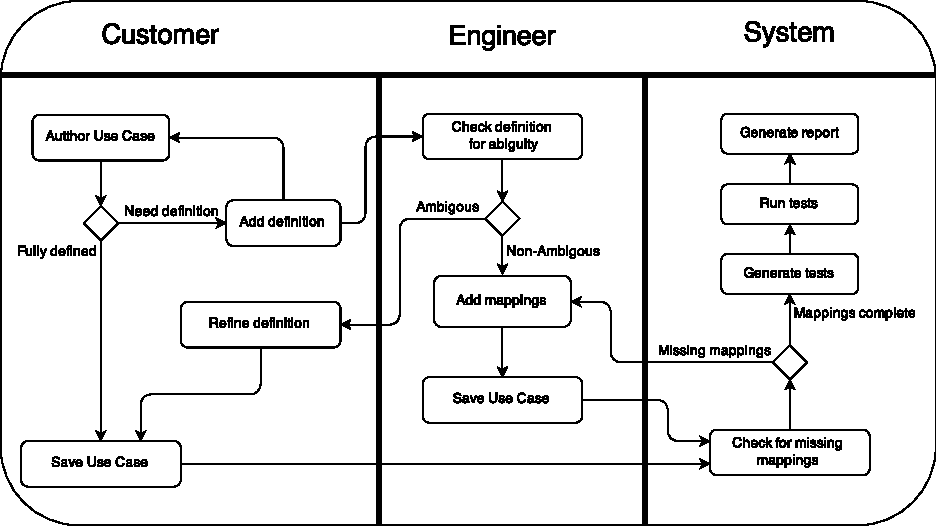
\includegraphics[scale=0.75]{img/use_case_creation_activity_diagram}
\centering
\caption{Use case creation with different actors}
\label{fig:use_case_creation_activity_diagram}
\end{figure}

The basic idea is that sufficient structure in requirement formalization may enable tests to be generated directly from requirements fully automatically. To facilitate this, it means that requirements should be written with a strong focus on testability, and try to avoid bad requirements. This, as a side effect, may increase the motivation for quantifying, constraining and refining requirements. As an example: \emph{Who} will perform this action, and how are the outcomes expected to be presented/received?\\\\
These questions should -- preferably -- be answered by the customer of the system, and mapped to actual functionality that may then be tested with regards to the behavior described in the requirements. So, in essence, the very basic use case; ``Administrator creates a new user'' with the postcondition ``The new user is created in the system'' should result in a test that, in some way, performs the ``add user'' action of the Administrator actor, and then verifies it against the postconditions. Ideally; with an appropriate level of detail provided in the use cases, and a grain of automated (and manual) mapping to domain concepts will enable automatic generation of acceptance tests. These can then be combined with a continuous integration service that runs the tests and reports results to developers.\\\\
The project will use the requirements from an existing system as a case study and formalize the structure of these, so that test generation from them is possible. During this process, we will investigate how to structure requirements so that we can generate tests directly from them and map implementation to requirements. Ideally, we want to identify general patterns and constraints in the structure/formalism introduced to our requirements in the case study, to be able to apply them to other projects. But in general, we will investigate to which extent this idea can be applied, and try to implement a translation tool that is able to translate a representation of a use cases into a tests case.

This thesis uses the software project ``OpenReception'' as case study. The project aims to provide a drop-in replacement for an existing system, and therefore has relatively fixed requirements that are extracted from the workings of the existing system. The system is developed and released under an open source license and any implementation details are therefore public domain and not covered by any non-disclosure agreements. \\\\
The project is, considered an extension of the test-driven development methodology, lifting it from its typical application of integration testing onto the new level of acceptance testing. This process is meant to be tool-assisted, so that tests may be generated automatically, but the mappings to the system needs to be done by hand.